\subsubsection{Datenbankplanung}
Als erstes musste ein passendes Datenbankschema entworfen werden, in dem die Sensordaten passend gespeichert werden können. Das folgende Schema stellt die Datenbankstruktur vor.
\begin{figure}[H]
	\centering
	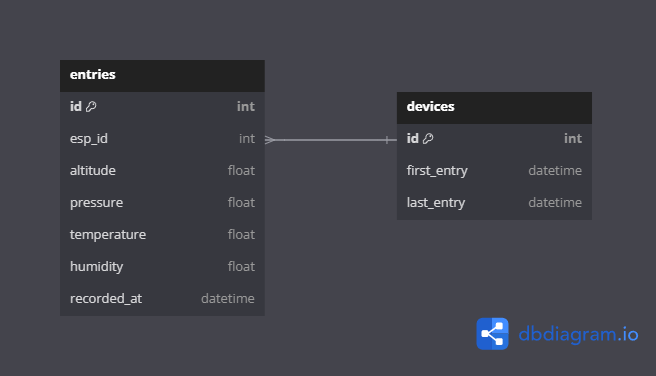
\includegraphics[width=15cm]{images/db_diagram.png}
	\caption{Datenbankdiagramm}
	\label{fig:db_diagram}
\end{figure}
Die Tabelle "`entries"' enthält die Messdaten, Höhe über N.N., den Luftdruck, die Temperatur, die Luftfeuchtigkeit und einen Zeitstempel des Messzeitpunktes, welche das Backend vom MQTT-Broker erhält. Außerdem wurde die Datenbank um eine Tabelle "`devices"' erweitert. Diese Tabelle speichert die einzigartigen Geräte, welche Daten in die Datenbank gespeichert haben. Sie enthält die "`ESP\_ID"' im Feld id, den ersten und letzten Eintrag des Geräts.

\subsubsection{Einrichtung der Datenbank}
Die MariaDB Datenbank wurde durch ein Script initialisiert.  Dieses sollte nur ein einziges mal, vor Inbetriebnahme des Systems ausgeführt werden, da durch Zeile eins, "`DROP DATABASE esp\_data;"', die Datenbank und alle in ihr enthaltenen Daten gelöscht werden. 
\begin{figure}[H]
	\centering
	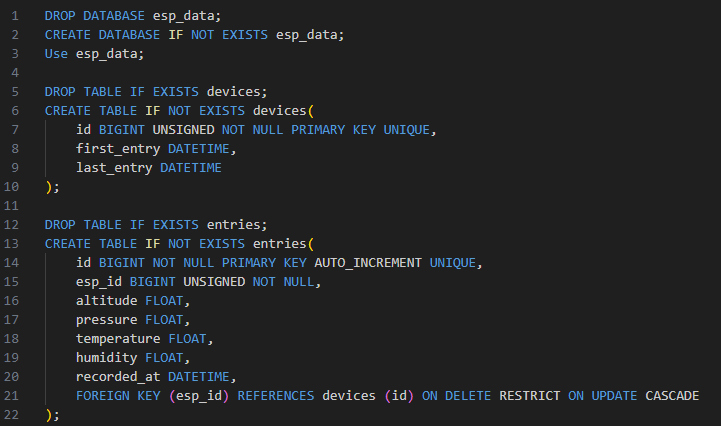
\includegraphics[width=15cm]{images/db_initialisation_script.png}
	\caption{Datenbankinitialisierungsscript}
	\label{fig:db_initialisation_script}
\end{figure}